\documentclass[1p]{elsarticle_modified}
%\bibliographystyle{elsarticle-num}

%\usepackage[colorlinks]{hyperref}
%\usepackage{abbrmath_seonhwa} %\Abb, \Ascr, \Acal ,\Abf, \Afrak
\usepackage{amsfonts}
\usepackage{amssymb}
\usepackage{amsmath}
\usepackage{amsthm}
\usepackage{scalefnt}
\usepackage{amsbsy}
\usepackage{kotex}
\usepackage{caption}
\usepackage{subfig}
\usepackage{color}
\usepackage{graphicx}
\usepackage{xcolor} %% white, black, red, green, blue, cyan, magenta, yellow
\usepackage{float}
\usepackage{setspace}
\usepackage{hyperref}

\usepackage{tikz}
\usetikzlibrary{arrows}

\usepackage{multirow}
\usepackage{array} % fixed length table
\usepackage{hhline}

%%%%%%%%%%%%%%%%%%%%%
\makeatletter
\renewcommand*\env@matrix[1][\arraystretch]{%
	\edef\arraystretch{#1}%
	\hskip -\arraycolsep
	\let\@ifnextchar\new@ifnextchar
	\array{*\c@MaxMatrixCols c}}
\makeatother %https://tex.stackexchange.com/questions/14071/how-can-i-increase-the-line-spacing-in-a-matrix
%%%%%%%%%%%%%%%

\usepackage[normalem]{ulem}

\newcommand{\msout}[1]{\ifmmode\text{\sout{\ensuremath{#1}}}\else\sout{#1}\fi}
%SOURCE: \msout is \stkout macro in https://tex.stackexchange.com/questions/20609/strikeout-in-math-mode

\newcommand{\cancel}[1]{
	\ifmmode
	{\color{red}\msout{#1}}
	\else
	{\color{red}\sout{#1}}
	\fi
}

\newcommand{\add}[1]{
	{\color{blue}\uwave{#1}}
}

\newcommand{\replace}[2]{
	\ifmmode
	{\color{red}\msout{#1}}{\color{blue}\uwave{#2}}
	\else
	{\color{red}\sout{#1}}{\color{blue}\uwave{#2}}
	\fi
}

\newcommand{\Sol}{\mathcal{S}} %segment
\newcommand{\D}{D} %diagram
\newcommand{\A}{\mathcal{A}} %arc


%%%%%%%%%%%%%%%%%%%%%%%%%%%%%5 test

\def\sl{\operatorname{\textup{SL}}(2,\Cbb)}
\def\psl{\operatorname{\textup{PSL}}(2,\Cbb)}
\def\quan{\mkern 1mu \triangleright \mkern 1mu}

\theoremstyle{definition}
\newtheorem{thm}{Theorem}[section]
\newtheorem{prop}[thm]{Proposition}
\newtheorem{lem}[thm]{Lemma}
\newtheorem{ques}[thm]{Question}
\newtheorem{cor}[thm]{Corollary}
\newtheorem{defn}[thm]{Definition}
\newtheorem{exam}[thm]{Example}
\newtheorem{rmk}[thm]{Remark}
\newtheorem{alg}[thm]{Algorithm}

\newcommand{\I}{\sqrt{-1}}
\begin{document}

%\begin{frontmatter}
%
%\title{Boundary parabolic representations of knots up to 8 crossings}
%
%%% Group authors per affiliation:
%\author{Yunhi Cho} 
%\address{Department of Mathematics, University of Seoul, Seoul, Korea}
%\ead{yhcho@uos.ac.kr}
%
%
%\author{Seonhwa Kim} %\fnref{s_kim}}
%\address{Center for Geometry and Physics, Institute for Basic Science, Pohang, 37673, Korea}
%\ead{ryeona17@ibs.re.kr}
%
%\author{Hyuk Kim}
%\address{Department of Mathematical Sciences, Seoul National University, Seoul 08826, Korea}
%\ead{hyukkim@snu.ac.kr}
%
%\author{Seokbeom Yoon}
%\address{Department of Mathematical Sciences, Seoul National University, Seoul, 08826,  Korea}
%\ead{sbyoon15@snu.ac.kr}
%
%\begin{abstract}
%We find all boundary parabolic representation of knots up to 8 crossings.
%
%\end{abstract}
%\begin{keyword}
%    \MSC[2010] 57M25 
%\end{keyword}
%
%\end{frontmatter}

%\linenumbers
%\tableofcontents
%
\newcommand\colored[1]{\textcolor{white}{\rule[-0.35ex]{0.8em}{1.4ex}}\kern-0.8em\color{red} #1}%
%\newcommand\colored[1]{\textcolor{white}{ #1}\kern-2.17ex	\textcolor{white}{ #1}\kern-1.81ex	\textcolor{white}{ #1}\kern-2.15ex\color{red}#1	}

{\Large $\underline{12n_{0476}~(K12n_{0476})}$}

\setlength{\tabcolsep}{10pt}
\renewcommand{\arraystretch}{1.6}
\vspace{1cm}\begin{tabular}{m{100pt}>{\centering\arraybackslash}m{274pt}}
\multirow{5}{120pt}{
	\centering
	\includegraphics[width=112pt]{../../../GIT/diagram.site/Diagrams/png/2565_12n_0476.png}\\
\ \ \ A knot diagram\footnotemark}&
\allowdisplaybreaks
\textbf{Linearized knot diagam} \\
\cline{2-2}
 &
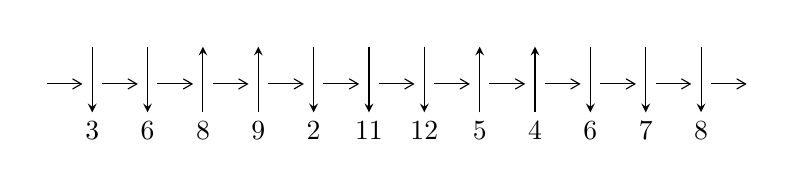
\begin{tikzpicture}[x=20pt, y=17pt]
	% nodes
	\node (C0) at (0, 0) {};
	\node (C1) at (1, 0) {};
	\node (C1U) at (1, +1) {};
	\node (C1D) at (1, -1) {3};

	\node (C2) at (2, 0) {};
	\node (C2U) at (2, +1) {};
	\node (C2D) at (2, -1) {6};

	\node (C3) at (3, 0) {};
	\node (C3U) at (3, +1) {};
	\node (C3D) at (3, -1) {8};

	\node (C4) at (4, 0) {};
	\node (C4U) at (4, +1) {};
	\node (C4D) at (4, -1) {9};

	\node (C5) at (5, 0) {};
	\node (C5U) at (5, +1) {};
	\node (C5D) at (5, -1) {2};

	\node (C6) at (6, 0) {};
	\node (C6U) at (6, +1) {};
	\node (C6D) at (6, -1) {11};

	\node (C7) at (7, 0) {};
	\node (C7U) at (7, +1) {};
	\node (C7D) at (7, -1) {12};

	\node (C8) at (8, 0) {};
	\node (C8U) at (8, +1) {};
	\node (C8D) at (8, -1) {5};

	\node (C9) at (9, 0) {};
	\node (C9U) at (9, +1) {};
	\node (C9D) at (9, -1) {4};

	\node (C10) at (10, 0) {};
	\node (C10U) at (10, +1) {};
	\node (C10D) at (10, -1) {6};

	\node (C11) at (11, 0) {};
	\node (C11U) at (11, +1) {};
	\node (C11D) at (11, -1) {7};

	\node (C12) at (12, 0) {};
	\node (C12U) at (12, +1) {};
	\node (C12D) at (12, -1) {8};
	\node (C13) at (13, 0) {};

	% arrows
	\draw[->,>={angle 60}]
	(C0) edge (C1) (C1) edge (C2) (C2) edge (C3) (C3) edge (C4) (C4) edge (C5) (C5) edge (C6) (C6) edge (C7) (C7) edge (C8) (C8) edge (C9) (C9) edge (C10) (C10) edge (C11) (C11) edge (C12) (C12) edge (C13) ;	\draw[->,>=stealth]
	(C1U) edge (C1D) (C2U) edge (C2D) (C3D) edge (C3U) (C4D) edge (C4U) (C5U) edge (C5D) (C6U) edge (C6D) (C7U) edge (C7D) (C8D) edge (C8U) (C9D) edge (C9U) (C10U) edge (C10D) (C11U) edge (C11D) (C12U) edge (C12D) ;
	\end{tikzpicture} \\
\hhline{~~} \\& 
\textbf{Solving Sequence} \\ \cline{2-2} 
 &
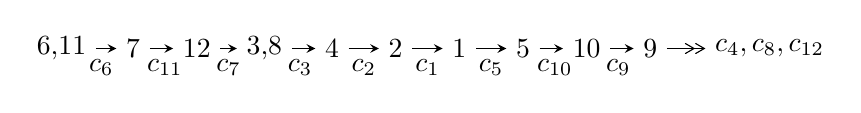
\begin{tikzpicture}[x=23pt, y=7pt]
	% node
	\node (A0) at (-1/8, 0) {6,11};
	\node (A1) at (1, 0) {7};
	\node (A2) at (2, 0) {12};
	\node (A3) at (49/16, 0) {3,8};
	\node (A4) at (33/8, 0) {4};
	\node (A5) at (41/8, 0) {2};
	\node (A6) at (49/8, 0) {1};
	\node (A7) at (57/8, 0) {5};
	\node (A8) at (65/8, 0) {10};
	\node (A9) at (73/8, 0) {9};
	\node (C1) at (1/2, -1) {$c_{6}$};
	\node (C2) at (3/2, -1) {$c_{11}$};
	\node (C3) at (5/2, -1) {$c_{7}$};
	\node (C4) at (29/8, -1) {$c_{3}$};
	\node (C5) at (37/8, -1) {$c_{2}$};
	\node (C6) at (45/8, -1) {$c_{1}$};
	\node (C7) at (53/8, -1) {$c_{5}$};
	\node (C8) at (61/8, -1) {$c_{10}$};
	\node (C9) at (69/8, -1) {$c_{9}$};
	\node (A10) at (11, 0) {$c_{4},c_{8},c_{12}$};

	% edge
	\draw[->,>=stealth]	
	(A0) edge (A1) (A1) edge (A2) (A2) edge (A3) (A3) edge (A4) (A4) edge (A5) (A5) edge (A6) (A6) edge (A7) (A7) edge (A8) (A8) edge (A9) ;
	\draw[->>,>={angle 60}]	
	(A9) edge (A10);
\end{tikzpicture} \\ 

\end{tabular} \\

\footnotetext{
The image of knot diagram is generated by the software ``\textbf{Draw programme}" developed by Andrew Bartholomew(\url{http://www.layer8.co.uk/maths/draw/index.htm\#Running-draw}), where we modified some parts for our purpose(\url{https://github.com/CATsTAILs/LinksPainter}).
}\phantom \\ \newline 
\centering \textbf{Ideals for irreducible components\footnotemark of $X_{\text{par}}$} 
 
\begin{align*}
I^u_{1}&=\langle 
-399369286162 u^{41}-497609046536 u^{40}+\cdots+724090717741 b-733512526727,\\
\phantom{I^u_{1}}&\phantom{= \langle  }-1720004901137 u^{41}+81273516863 u^{40}+\cdots+4344544306446 a-9063190310470,\\
\phantom{I^u_{1}}&\phantom{= \langle  }u^{42}+2 u^{41}+\cdots- u+3\rangle \\
I^u_{2}&=\langle 
b-1,\;a^2-2 a-2 u+5,\;u^2- u-1\rangle \\
I^u_{3}&=\langle 
b+1,\;a+1,\;u^2+u-1\rangle \\
\\
\end{align*}
\raggedright * 3 irreducible components of $\dim_{\mathbb{C}}=0$, with total 48 representations.\\
\footnotetext{All coefficients of polynomials are rational numbers. But the coefficients are sometimes approximated in decimal forms when there is not enough margin.}
\newpage
\renewcommand{\arraystretch}{1}
\centering \section*{I. $I^u_{1}= \langle -3.99\times10^{11} u^{41}-4.98\times10^{11} u^{40}+\cdots+7.24\times10^{11} b-7.34\times10^{11},\;-1.72\times10^{12} u^{41}+8.13\times10^{10} u^{40}+\cdots+4.34\times10^{12} a-9.06\times10^{12},\;u^{42}+2 u^{41}+\cdots- u+3 \rangle$}
\flushleft \textbf{(i) Arc colorings}\\
\begin{tabular}{m{7pt} m{180pt} m{7pt} m{180pt} }
\flushright $a_{6}=$&$\begin{pmatrix}1\\0\end{pmatrix}$ \\
\flushright $a_{11}=$&$\begin{pmatrix}0\\u\end{pmatrix}$ \\
\flushright $a_{7}=$&$\begin{pmatrix}1\\u^2\end{pmatrix}$ \\
\flushright $a_{12}=$&$\begin{pmatrix}- u\\- u^3+u\end{pmatrix}$ \\
\flushright $a_{3}=$&$\begin{pmatrix}0.395900 u^{41}-0.0187070 u^{40}+\cdots-2.07593 u+2.08611\\0.551546 u^{41}+0.687219 u^{40}+\cdots-1.66740 u+1.01301\end{pmatrix}$ \\
\flushright $a_{8}=$&$\begin{pmatrix}- u^2+1\\- u^4+2 u^2\end{pmatrix}$ \\
\flushright $a_{4}=$&$\begin{pmatrix}0.816087 u^{41}+0.338018 u^{40}+\cdots-4.06896 u+3.36970\\0.759348 u^{41}+0.839252 u^{40}+\cdots-2.61706 u+1.37583\end{pmatrix}$ \\
\flushright $a_{2}=$&$\begin{pmatrix}0.947446 u^{41}+0.668512 u^{40}+\cdots-3.74333 u+3.09912\\0.551546 u^{41}+0.687219 u^{40}+\cdots-1.66740 u+1.01301\end{pmatrix}$ \\
\flushright $a_{1}=$&$\begin{pmatrix}u^3-2 u\\u^5-3 u^3+u\end{pmatrix}$ \\
\flushright $a_{5}=$&$\begin{pmatrix}0.835547 u^{41}+0.380630 u^{40}+\cdots+6.27378 u+0.289814\\0.900701 u^{41}+0.654885 u^{40}+\cdots+0.388683 u+1.42313\end{pmatrix}$ \\
\flushright $a_{10}=$&$\begin{pmatrix}u\\u\end{pmatrix}$ \\
\flushright $a_{9}=$&$\begin{pmatrix}0.988524 u^{41}+0.535525 u^{40}+\cdots-1.74947 u+4.21201\\0.136440 u^{41}+0.143354 u^{40}+\cdots+0.793437 u+1.35900\end{pmatrix}$\\&\end{tabular}
\flushleft \textbf{(ii) Obstruction class $= -1$}\\~\\
\flushleft \textbf{(iii) Cusp Shapes $= \frac{784004418607}{724090717741} u^{41}+\frac{2116932802003}{724090717741} u^{40}+\cdots-\frac{5911721578314}{724090717741} u-\frac{3580528018791}{724090717741}$}\\~\\
\newpage\renewcommand{\arraystretch}{1}
\flushleft \textbf{(iv) u-Polynomials at the component}\newline \\
\begin{tabular}{m{50pt}|m{274pt}}
Crossings & \hspace{64pt}u-Polynomials at each crossing \\
\hline $$\begin{aligned}c_{1}\end{aligned}$$&$\begin{aligned}
&u^{42}+17 u^{41}+\cdots+1720 u+121
\end{aligned}$\\
\hline $$\begin{aligned}c_{2},c_{5}\end{aligned}$$&$\begin{aligned}
&u^{42}+3 u^{41}+\cdots+24 u+11
\end{aligned}$\\
\hline $$\begin{aligned}c_{3}\end{aligned}$$&$\begin{aligned}
&u^{42}+u^{41}+\cdots-160 u+100
\end{aligned}$\\
\hline $$\begin{aligned}c_{4},c_{8},c_{9}\end{aligned}$$&$\begin{aligned}
&u^{42}- u^{41}+\cdots-32 u^2+4
\end{aligned}$\\
\hline $$\begin{aligned}c_{6},c_{7},c_{10}\\c_{11},c_{12}\end{aligned}$$&$\begin{aligned}
&u^{42}-2 u^{41}+\cdots+u+3
\end{aligned}$\\
\hline
\end{tabular}\\~\\
\newpage\renewcommand{\arraystretch}{1}
\flushleft \textbf{(v) Riley Polynomials at the component}\newline \\
\begin{tabular}{m{50pt}|m{274pt}}
Crossings & \hspace{64pt}Riley Polynomials at each crossing \\
\hline $$\begin{aligned}c_{1}\end{aligned}$$&$\begin{aligned}
&y^{42}+23 y^{41}+\cdots+258748 y+14641
\end{aligned}$\\
\hline $$\begin{aligned}c_{2},c_{5}\end{aligned}$$&$\begin{aligned}
&y^{42}-17 y^{41}+\cdots-1720 y+121
\end{aligned}$\\
\hline $$\begin{aligned}c_{3}\end{aligned}$$&$\begin{aligned}
&y^{42}-23 y^{41}+\cdots-179200 y+10000
\end{aligned}$\\
\hline $$\begin{aligned}c_{4},c_{8},c_{9}\end{aligned}$$&$\begin{aligned}
&y^{42}+37 y^{41}+\cdots-256 y+16
\end{aligned}$\\
\hline $$\begin{aligned}c_{6},c_{7},c_{10}\\c_{11},c_{12}\end{aligned}$$&$\begin{aligned}
&y^{42}-48 y^{41}+\cdots-115 y+9
\end{aligned}$\\
\hline
\end{tabular}\\~\\
\newpage\flushleft \textbf{(vi) Complex Volumes and Cusp Shapes}
$$\begin{array}{c|c|c}  
\text{Solutions to }I^u_{1}& \I (\text{vol} + \sqrt{-1}CS) & \text{Cusp shape}\\
 \hline 
\begin{aligned}
u &= -1.049280 + 0.091551 I \\
a &= \phantom{-}0.412704 - 0.129591 I \\
b &= \phantom{-}0.776169 + 0.605347 I\end{aligned}
 & -4.77432 - 2.23397 I & -10.46787 + 3.24456 I \\ \hline\begin{aligned}
u &= -1.049280 - 0.091551 I \\
a &= \phantom{-}0.412704 + 0.129591 I \\
b &= \phantom{-}0.776169 - 0.605347 I\end{aligned}
 & -4.77432 + 2.23397 I & -10.46787 - 3.24456 I \\ \hline\begin{aligned}
u &= \phantom{-}0.673657 + 0.613325 I \\
a &= \phantom{-}0.46793 - 1.91116 I \\
b &= \phantom{-}1.100550 + 0.724909 I\end{aligned}
 & -1.23257 - 9.56169 I & -8.38946 + 7.95988 I \\ \hline\begin{aligned}
u &= \phantom{-}0.673657 - 0.613325 I \\
a &= \phantom{-}0.46793 + 1.91116 I \\
b &= \phantom{-}1.100550 - 0.724909 I\end{aligned}
 & -1.23257 + 9.56169 I & -8.38946 - 7.95988 I \\ \hline\begin{aligned}
u &= -0.576900 + 0.629034 I \\
a &= -0.25109 - 1.86774 I \\
b &= -0.957258 + 0.776390 I\end{aligned}
 & \phantom{-}3.58322 + 5.14982 I & -3.56640 - 6.23803 I \\ \hline\begin{aligned}
u &= -0.576900 - 0.629034 I \\
a &= -0.25109 + 1.86774 I \\
b &= -0.957258 - 0.776390 I\end{aligned}
 & \phantom{-}3.58322 - 5.14982 I & -3.56640 + 6.23803 I \\ \hline\begin{aligned}
u &= \phantom{-}0.553857 + 0.616758 I \\
a &= -0.988096 + 0.680405 I \\
b &= \phantom{-}0.572226 - 0.890720 I\end{aligned}
 & \phantom{-}0.35890 - 3.56775 I & -5.83599 + 3.90838 I \\ \hline\begin{aligned}
u &= \phantom{-}0.553857 - 0.616758 I \\
a &= -0.988096 - 0.680405 I \\
b &= \phantom{-}0.572226 + 0.890720 I\end{aligned}
 & \phantom{-}0.35890 + 3.56775 I & -5.83599 - 3.90838 I \\ \hline\begin{aligned}
u &= \phantom{-}0.786427\phantom{ +0.000000I} \\
a &= -0.785424\phantom{ +0.000000I} \\
b &= -0.488406\phantom{ +0.000000I}\end{aligned}
 & -1.56406\phantom{ +0.000000I} & -3.83480\phantom{ +0.000000I} \\ \hline\begin{aligned}
u &= -0.415353 + 0.654172 I \\
a &= \phantom{-}0.983300 + 0.831773 I \\
b &= -0.801220 - 0.815689 I\end{aligned}
 & \phantom{-}4.05957 - 0.81400 I & -1.93866 - 0.14480 I\\
 \hline 
 \end{array}$$\newpage$$\begin{array}{c|c|c}  
\text{Solutions to }I^u_{1}& \I (\text{vol} + \sqrt{-1}CS) & \text{Cusp shape}\\
 \hline 
\begin{aligned}
u &= -0.415353 - 0.654172 I \\
a &= \phantom{-}0.983300 - 0.831773 I \\
b &= -0.801220 + 0.815689 I\end{aligned}
 & \phantom{-}4.05957 + 0.81400 I & -1.93866 + 0.14480 I \\ \hline\begin{aligned}
u &= \phantom{-}0.430526 + 0.624525 I \\
a &= -0.00031 - 1.73658 I \\
b &= \phantom{-}0.721316 + 0.800712 I\end{aligned}
 & \phantom{-}0.718852 - 0.648201 I & -5.19720 + 2.33460 I \\ \hline\begin{aligned}
u &= \phantom{-}0.430526 - 0.624525 I \\
a &= -0.00031 + 1.73658 I \\
b &= \phantom{-}0.721316 - 0.800712 I\end{aligned}
 & \phantom{-}0.718852 + 0.648201 I & -5.19720 - 2.33460 I \\ \hline\begin{aligned}
u &= \phantom{-}0.289860 + 0.689463 I \\
a &= -0.902818 + 0.978781 I \\
b &= \phantom{-}0.995362 - 0.745920 I\end{aligned}
 & -0.10093 + 5.18138 I & -5.92756 - 3.03712 I \\ \hline\begin{aligned}
u &= \phantom{-}0.289860 - 0.689463 I \\
a &= -0.902818 - 0.978781 I \\
b &= \phantom{-}0.995362 + 0.745920 I\end{aligned}
 & -0.10093 - 5.18138 I & -5.92756 + 3.03712 I \\ \hline\begin{aligned}
u &= -1.333380 + 0.055601 I \\
a &= \phantom{-}0.083600 - 0.453941 I \\
b &= \phantom{-}0.713786 + 0.763955 I\end{aligned}
 & -4.90307 - 2.25991 I & \phantom{-0.000000 } 0 \\ \hline\begin{aligned}
u &= -1.333380 - 0.055601 I \\
a &= \phantom{-}0.083600 + 0.453941 I \\
b &= \phantom{-}0.713786 - 0.763955 I\end{aligned}
 & -4.90307 + 2.25991 I & \phantom{-0.000000 } 0 \\ \hline\begin{aligned}
u &= \phantom{-}0.476375 + 0.392459 I \\
a &= -0.604894 + 0.926643 I \\
b &= -1.261030 + 0.067596 I\end{aligned}
 & -6.08478 - 1.41154 I & -9.66825 + 4.90149 I \\ \hline\begin{aligned}
u &= \phantom{-}0.476375 - 0.392459 I \\
a &= -0.604894 - 0.926643 I \\
b &= -1.261030 - 0.067596 I\end{aligned}
 & -6.08478 + 1.41154 I & -9.66825 - 4.90149 I \\ \hline\begin{aligned}
u &= -0.475739 + 0.258622 I \\
a &= \phantom{-}1.77841 - 2.91372 I \\
b &= -0.798648 + 0.217030 I\end{aligned}
 & -6.83314 + 0.96606 I & -8.00205 - 7.45219 I\\
 \hline 
 \end{array}$$\newpage$$\begin{array}{c|c|c}  
\text{Solutions to }I^u_{1}& \I (\text{vol} + \sqrt{-1}CS) & \text{Cusp shape}\\
 \hline 
\begin{aligned}
u &= -0.475739 - 0.258622 I \\
a &= \phantom{-}1.77841 + 2.91372 I \\
b &= -0.798648 - 0.217030 I\end{aligned}
 & -6.83314 - 0.96606 I & -8.00205 + 7.45219 I \\ \hline\begin{aligned}
u &= \phantom{-}1.45883 + 0.17891 I \\
a &= \phantom{-}0.245004 - 0.259927 I \\
b &= -0.587321 + 0.900636 I\end{aligned}
 & -1.96643 - 2.13199 I & \phantom{-0.000000 } 0 \\ \hline\begin{aligned}
u &= \phantom{-}1.45883 - 0.17891 I \\
a &= \phantom{-}0.245004 + 0.259927 I \\
b &= -0.587321 - 0.900636 I\end{aligned}
 & -1.96643 + 2.13199 I & \phantom{-0.000000 } 0 \\ \hline\begin{aligned}
u &= -1.48695 + 0.16260 I \\
a &= \phantom{-}0.560834 + 1.090920 I \\
b &= \phantom{-}0.940796 - 0.731217 I\end{aligned}
 & -5.49810 + 3.38316 I & \phantom{-0.000000 } 0 \\ \hline\begin{aligned}
u &= -1.48695 - 0.16260 I \\
a &= \phantom{-}0.560834 - 1.090920 I \\
b &= \phantom{-}0.940796 + 0.731217 I\end{aligned}
 & -5.49810 - 3.38316 I & \phantom{-0.000000 } 0 \\ \hline\begin{aligned}
u &= \phantom{-}1.51893\phantom{ +0.000000I} \\
a &= \phantom{-}1.19880\phantom{ +0.000000I} \\
b &= \phantom{-}1.30296\phantom{ +0.000000I}\end{aligned}
 & -8.88024\phantom{ +0.000000I} & \phantom{-0.000000 } 0 \\ \hline\begin{aligned}
u &= -1.53094 + 0.09497 I \\
a &= -1.171830 - 0.180431 I \\
b &= -1.351610 - 0.153172 I\end{aligned}
 & -12.84770 + 3.06597 I & \phantom{-0.000000 } 0 \\ \hline\begin{aligned}
u &= -1.53094 - 0.09497 I \\
a &= -1.171830 + 0.180431 I \\
b &= -1.351610 + 0.153172 I\end{aligned}
 & -12.84770 - 3.06597 I & \phantom{-0.000000 } 0 \\ \hline\begin{aligned}
u &= \phantom{-}1.53459 + 0.05929 I \\
a &= \phantom{-}0.06391 + 1.58702 I \\
b &= -0.843652 - 0.499599 I\end{aligned}
 & -13.66930 - 2.02433 I & \phantom{-0.000000 } 0 \\ \hline\begin{aligned}
u &= \phantom{-}1.53459 - 0.05929 I \\
a &= \phantom{-}0.06391 - 1.58702 I \\
b &= -0.843652 + 0.499599 I\end{aligned}
 & -13.66930 + 2.02433 I & \phantom{-0.000000 } 0\\
 \hline 
 \end{array}$$\newpage$$\begin{array}{c|c|c}  
\text{Solutions to }I^u_{1}& \I (\text{vol} + \sqrt{-1}CS) & \text{Cusp shape}\\
 \hline 
\begin{aligned}
u &= -1.53944 + 0.19194 I \\
a &= -0.385692 - 0.184391 I \\
b &= \phantom{-}0.433918 + 0.972193 I\end{aligned}
 & -6.56394 + 6.51432 I & \phantom{-0.000000 } 0 \\ \hline\begin{aligned}
u &= -1.53944 - 0.19194 I \\
a &= -0.385692 + 0.184391 I \\
b &= \phantom{-}0.433918 - 0.972193 I\end{aligned}
 & -6.56394 - 6.51432 I & \phantom{-0.000000 } 0 \\ \hline\begin{aligned}
u &= \phantom{-}1.55140 + 0.19874 I \\
a &= -0.84494 + 1.14482 I \\
b &= -1.088960 - 0.737531 I\end{aligned}
 & -3.47009 - 8.18357 I & \phantom{-0.000000 } 0 \\ \hline\begin{aligned}
u &= \phantom{-}1.55140 - 0.19874 I \\
a &= -0.84494 - 1.14482 I \\
b &= -1.088960 + 0.737531 I\end{aligned}
 & -3.47009 + 8.18357 I & \phantom{-0.000000 } 0 \\ \hline\begin{aligned}
u &= -0.425520\phantom{ +0.000000I} \\
a &= \phantom{-}1.66207\phantom{ +0.000000I} \\
b &= \phantom{-}1.09128\phantom{ +0.000000I}\end{aligned}
 & -2.26322\phantom{ +0.000000I} & \phantom{-}5.01380\phantom{ +0.000000I} \\ \hline\begin{aligned}
u &= \phantom{-}0.242324 + 0.345213 I \\
a &= -0.599361 - 1.192230 I \\
b &= \phantom{-}0.361519 + 0.367349 I\end{aligned}
 & -0.227692 - 0.948273 I & -4.31648 + 7.21437 I \\ \hline\begin{aligned}
u &= \phantom{-}0.242324 - 0.345213 I \\
a &= -0.599361 + 1.192230 I \\
b &= \phantom{-}0.361519 - 0.367349 I\end{aligned}
 & -0.227692 + 0.948273 I & -4.31648 - 7.21437 I \\ \hline\begin{aligned}
u &= -1.59476 + 0.19372 I \\
a &= \phantom{-}1.02426 + 1.19954 I \\
b &= \phantom{-}1.179170 - 0.691260 I\end{aligned}
 & -8.8337 + 12.5829 I & \phantom{-0.000000 } 0 \\ \hline\begin{aligned}
u &= -1.59476 - 0.19372 I \\
a &= \phantom{-}1.02426 - 1.19954 I \\
b &= \phantom{-}1.179170 + 0.691260 I\end{aligned}
 & -8.8337 - 12.5829 I & \phantom{-0.000000 } 0 \\ \hline\begin{aligned}
u &= -1.64206\phantom{ +0.000000I} \\
a &= -0.939257\phantom{ +0.000000I} \\
b &= -0.789120\phantom{ +0.000000I}\end{aligned}
 & -10.0738\phantom{ +0.000000I} & \phantom{-0.000000 } 0\\
 \hline 
 \end{array}$$\newpage$$\begin{array}{c|c|c}  
\text{Solutions to }I^u_{1}& \I (\text{vol} + \sqrt{-1}CS) & \text{Cusp shape}\\
 \hline 
\begin{aligned}
u &= \phantom{-}1.67244 + 0.02610 I \\
a &= \phantom{-}0.894316 - 0.090456 I \\
b &= \phantom{-}0.836517 - 0.423614 I\end{aligned}
 & -14.0854 + 1.7540 I & \phantom{-0.000000 } 0 \\ \hline\begin{aligned}
u &= \phantom{-}1.67244 - 0.02610 I \\
a &= \phantom{-}0.894316 + 0.090456 I \\
b &= \phantom{-}0.836517 + 0.423614 I\end{aligned}
 & -14.0854 - 1.7540 I & \phantom{-0.000000 } 0\\
 \hline 
 \end{array}$$\newpage\newpage\renewcommand{\arraystretch}{1}
\centering \section*{II. $I^u_{2}= \langle b-1,\;a^2-2 a-2 u+5,\;u^2- u-1 \rangle$}
\flushleft \textbf{(i) Arc colorings}\\
\begin{tabular}{m{7pt} m{180pt} m{7pt} m{180pt} }
\flushright $a_{6}=$&$\begin{pmatrix}1\\0\end{pmatrix}$ \\
\flushright $a_{11}=$&$\begin{pmatrix}0\\u\end{pmatrix}$ \\
\flushright $a_{7}=$&$\begin{pmatrix}1\\u+1\end{pmatrix}$ \\
\flushright $a_{12}=$&$\begin{pmatrix}- u\\- u-1\end{pmatrix}$ \\
\flushright $a_{3}=$&$\begin{pmatrix}a\\1\end{pmatrix}$ \\
\flushright $a_{8}=$&$\begin{pmatrix}- u\\- u\end{pmatrix}$ \\
\flushright $a_{4}=$&$\begin{pmatrix}- a u+u+1\\- a u- a+u+2\end{pmatrix}$ \\
\flushright $a_{2}=$&$\begin{pmatrix}a+1\\1\end{pmatrix}$ \\
\flushright $a_{1}=$&$\begin{pmatrix}1\\0\end{pmatrix}$ \\
\flushright $a_{5}=$&$\begin{pmatrix}- a\\-1\end{pmatrix}$ \\
\flushright $a_{10}=$&$\begin{pmatrix}u\\u\end{pmatrix}$ \\
\flushright $a_{9}=$&$\begin{pmatrix}- a u+2 u-2\\- a u\end{pmatrix}$\\&\end{tabular}
\flushleft \textbf{(ii) Obstruction class $= 1$}\\~\\
\flushleft \textbf{(iii) Cusp Shapes $= -16$}\\~\\
\newpage\renewcommand{\arraystretch}{1}
\flushleft \textbf{(iv) u-Polynomials at the component}\newline \\
\begin{tabular}{m{50pt}|m{274pt}}
Crossings & \hspace{64pt}u-Polynomials at each crossing \\
\hline $$\begin{aligned}c_{1},c_{5}\end{aligned}$$&$\begin{aligned}
&(u-1)^4
\end{aligned}$\\
\hline $$\begin{aligned}c_{2}\end{aligned}$$&$\begin{aligned}
&(u+1)^4
\end{aligned}$\\
\hline $$\begin{aligned}c_{3},c_{4},c_{8}\\c_{9}\end{aligned}$$&$\begin{aligned}
&(u^2+2)^2
\end{aligned}$\\
\hline $$\begin{aligned}c_{6},c_{7}\end{aligned}$$&$\begin{aligned}
&(u^2- u-1)^2
\end{aligned}$\\
\hline $$\begin{aligned}c_{10},c_{11},c_{12}\end{aligned}$$&$\begin{aligned}
&(u^2+u-1)^2
\end{aligned}$\\
\hline
\end{tabular}\\~\\
\newpage\renewcommand{\arraystretch}{1}
\flushleft \textbf{(v) Riley Polynomials at the component}\newline \\
\begin{tabular}{m{50pt}|m{274pt}}
Crossings & \hspace{64pt}Riley Polynomials at each crossing \\
\hline $$\begin{aligned}c_{1},c_{2},c_{5}\end{aligned}$$&$\begin{aligned}
&(y-1)^4
\end{aligned}$\\
\hline $$\begin{aligned}c_{3},c_{4},c_{8}\\c_{9}\end{aligned}$$&$\begin{aligned}
&(y+2)^4
\end{aligned}$\\
\hline $$\begin{aligned}c_{6},c_{7},c_{10}\\c_{11},c_{12}\end{aligned}$$&$\begin{aligned}
&(y^2-3 y+1)^2
\end{aligned}$\\
\hline
\end{tabular}\\~\\
\newpage\flushleft \textbf{(vi) Complex Volumes and Cusp Shapes}
$$\begin{array}{c|c|c}  
\text{Solutions to }I^u_{2}& \I (\text{vol} + \sqrt{-1}CS) & \text{Cusp shape}\\
 \hline 
\begin{aligned}
u &= -0.618034\phantom{ +0.000000I} \\
a &= \phantom{-}1.00000 + 2.28825 I \\
b &= \phantom{-}1.00000\phantom{ +0.000000I}\end{aligned}
 & -7.56670\phantom{ +0.000000I} & -16.0000\phantom{ +0.000000I} \\ \hline\begin{aligned}
u &= -0.618034\phantom{ +0.000000I} \\
a &= \phantom{-}1.00000 - 2.28825 I \\
b &= \phantom{-}1.00000\phantom{ +0.000000I}\end{aligned}
 & -7.56670\phantom{ +0.000000I} & -16.0000\phantom{ +0.000000I} \\ \hline\begin{aligned}
u &= \phantom{-}1.61803\phantom{ +0.000000I} \\
a &= \phantom{-}1.000000 + 0.874032 I \\
b &= \phantom{-}1.00000\phantom{ +0.000000I}\end{aligned}
 & -15.4624\phantom{ +0.000000I} & -16.0000\phantom{ +0.000000I} \\ \hline\begin{aligned}
u &= \phantom{-}1.61803\phantom{ +0.000000I} \\
a &= \phantom{-}1.000000 - 0.874032 I \\
b &= \phantom{-}1.00000\phantom{ +0.000000I}\end{aligned}
 & -15.4624\phantom{ +0.000000I} & -16.0000\phantom{ +0.000000I}\\
 \hline 
 \end{array}$$\newpage\newpage\renewcommand{\arraystretch}{1}
\centering \section*{III. $I^u_{3}= \langle b+1,\;a+1,\;u^2+u-1 \rangle$}
\flushleft \textbf{(i) Arc colorings}\\
\begin{tabular}{m{7pt} m{180pt} m{7pt} m{180pt} }
\flushright $a_{6}=$&$\begin{pmatrix}1\\0\end{pmatrix}$ \\
\flushright $a_{11}=$&$\begin{pmatrix}0\\u\end{pmatrix}$ \\
\flushright $a_{7}=$&$\begin{pmatrix}1\\- u+1\end{pmatrix}$ \\
\flushright $a_{12}=$&$\begin{pmatrix}- u\\- u+1\end{pmatrix}$ \\
\flushright $a_{3}=$&$\begin{pmatrix}-1\\-1\end{pmatrix}$ \\
\flushright $a_{8}=$&$\begin{pmatrix}u\\u\end{pmatrix}$ \\
\flushright $a_{4}=$&$\begin{pmatrix}-1\\-1\end{pmatrix}$ \\
\flushright $a_{2}=$&$\begin{pmatrix}-2\\-1\end{pmatrix}$ \\
\flushright $a_{1}=$&$\begin{pmatrix}-1\\0\end{pmatrix}$ \\
\flushright $a_{5}=$&$\begin{pmatrix}-1\\-1\end{pmatrix}$ \\
\flushright $a_{10}=$&$\begin{pmatrix}u\\u\end{pmatrix}$ \\
\flushright $a_{9}=$&$\begin{pmatrix}u\\u\end{pmatrix}$\\&\end{tabular}
\flushleft \textbf{(ii) Obstruction class $= 1$}\\~\\
\flushleft \textbf{(iii) Cusp Shapes $= -18$}\\~\\
\newpage\renewcommand{\arraystretch}{1}
\flushleft \textbf{(iv) u-Polynomials at the component}\newline \\
\begin{tabular}{m{50pt}|m{274pt}}
Crossings & \hspace{64pt}u-Polynomials at each crossing \\
\hline $$\begin{aligned}c_{1},c_{2}\end{aligned}$$&$\begin{aligned}
&(u-1)^2
\end{aligned}$\\
\hline $$\begin{aligned}c_{3},c_{4},c_{8}\\c_{9}\end{aligned}$$&$\begin{aligned}
&u^2
\end{aligned}$\\
\hline $$\begin{aligned}c_{5}\end{aligned}$$&$\begin{aligned}
&(u+1)^2
\end{aligned}$\\
\hline $$\begin{aligned}c_{6},c_{7}\end{aligned}$$&$\begin{aligned}
&u^2+u-1
\end{aligned}$\\
\hline $$\begin{aligned}c_{10},c_{11},c_{12}\end{aligned}$$&$\begin{aligned}
&u^2- u-1
\end{aligned}$\\
\hline
\end{tabular}\\~\\
\newpage\renewcommand{\arraystretch}{1}
\flushleft \textbf{(v) Riley Polynomials at the component}\newline \\
\begin{tabular}{m{50pt}|m{274pt}}
Crossings & \hspace{64pt}Riley Polynomials at each crossing \\
\hline $$\begin{aligned}c_{1},c_{2},c_{5}\end{aligned}$$&$\begin{aligned}
&(y-1)^2
\end{aligned}$\\
\hline $$\begin{aligned}c_{3},c_{4},c_{8}\\c_{9}\end{aligned}$$&$\begin{aligned}
&y^2
\end{aligned}$\\
\hline $$\begin{aligned}c_{6},c_{7},c_{10}\\c_{11},c_{12}\end{aligned}$$&$\begin{aligned}
&y^2-3 y+1
\end{aligned}$\\
\hline
\end{tabular}\\~\\
\newpage\flushleft \textbf{(vi) Complex Volumes and Cusp Shapes}
$$\begin{array}{c|c|c}  
\text{Solutions to }I^u_{3}& \I (\text{vol} + \sqrt{-1}CS) & \text{Cusp shape}\\
 \hline 
\begin{aligned}
u &= \phantom{-}0.618034\phantom{ +0.000000I} \\
a &= -1.00000\phantom{ +0.000000I} \\
b &= -1.00000\phantom{ +0.000000I}\end{aligned}
 & -2.63189\phantom{ +0.000000I} & -18.0000\phantom{ +0.000000I} \\ \hline\begin{aligned}
u &= -1.61803\phantom{ +0.000000I} \\
a &= -1.00000\phantom{ +0.000000I} \\
b &= -1.00000\phantom{ +0.000000I}\end{aligned}
 & -10.5276\phantom{ +0.000000I} & -18.0000\phantom{ +0.000000I}\\
 \hline 
 \end{array}$$\newpage
\newpage\renewcommand{\arraystretch}{1}
\centering \section*{ IV. u-Polynomials}
\begin{tabular}{m{50pt}|m{274pt}}
Crossings & \hspace{64pt}u-Polynomials at each crossing \\
\hline $$\begin{aligned}c_{1}\end{aligned}$$&$\begin{aligned}
&((u-1)^6)(u^{42}+17 u^{41}+\cdots+1720 u+121)
\end{aligned}$\\
\hline $$\begin{aligned}c_{2}\end{aligned}$$&$\begin{aligned}
&((u-1)^2)(u+1)^4(u^{42}+3 u^{41}+\cdots+24 u+11)
\end{aligned}$\\
\hline $$\begin{aligned}c_{3}\end{aligned}$$&$\begin{aligned}
&u^2(u^2+2)^2(u^{42}+u^{41}+\cdots-160 u+100)
\end{aligned}$\\
\hline $$\begin{aligned}c_{4},c_{8},c_{9}\end{aligned}$$&$\begin{aligned}
&u^2(u^2+2)^2(u^{42}- u^{41}+\cdots-32 u^2+4)
\end{aligned}$\\
\hline $$\begin{aligned}c_{5}\end{aligned}$$&$\begin{aligned}
&((u-1)^4)(u+1)^2(u^{42}+3 u^{41}+\cdots+24 u+11)
\end{aligned}$\\
\hline $$\begin{aligned}c_{6},c_{7}\end{aligned}$$&$\begin{aligned}
&((u^2- u-1)^2)(u^2+u-1)(u^{42}-2 u^{41}+\cdots+u+3)
\end{aligned}$\\
\hline $$\begin{aligned}c_{10},c_{11},c_{12}\end{aligned}$$&$\begin{aligned}
&(u^2- u-1)(u^2+u-1)^2(u^{42}-2 u^{41}+\cdots+u+3)
\end{aligned}$\\
\hline
\end{tabular}\newpage\renewcommand{\arraystretch}{1}
\centering \section*{ V. Riley Polynomials}
\begin{tabular}{m{50pt}|m{274pt}}
Crossings & \hspace{64pt}Riley Polynomials at each crossing \\
\hline $$\begin{aligned}c_{1}\end{aligned}$$&$\begin{aligned}
&((y-1)^6)(y^{42}+23 y^{41}+\cdots+258748 y+14641)
\end{aligned}$\\
\hline $$\begin{aligned}c_{2},c_{5}\end{aligned}$$&$\begin{aligned}
&((y-1)^6)(y^{42}-17 y^{41}+\cdots-1720 y+121)
\end{aligned}$\\
\hline $$\begin{aligned}c_{3}\end{aligned}$$&$\begin{aligned}
&y^2(y+2)^4(y^{42}-23 y^{41}+\cdots-179200 y+10000)
\end{aligned}$\\
\hline $$\begin{aligned}c_{4},c_{8},c_{9}\end{aligned}$$&$\begin{aligned}
&y^2(y+2)^4(y^{42}+37 y^{41}+\cdots-256 y+16)
\end{aligned}$\\
\hline $$\begin{aligned}c_{6},c_{7},c_{10}\\c_{11},c_{12}\end{aligned}$$&$\begin{aligned}
&((y^2-3 y+1)^3)(y^{42}-48 y^{41}+\cdots-115 y+9)
\end{aligned}$\\
\hline
\end{tabular}
\vskip 2pc
\end{document}